\documentclass[tikz,border=6pt]{standalone}
\usepackage{pgfplots}
\pgfplotsset{compat=1.18}
\usepgfplotslibrary{colormaps}
\usetikzlibrary{arrows, arrows.meta, calc}

\usepackage{amssymb,amsmath,mathtools}

\usepackage[T1]{fontenc}
\usepackage[utf8]{inputenc}
\usepackage{newpxtext,newpxmath}
\usepackage{sectsty}

\renewcommand{\Re}{\mathrm{Re}}
\renewcommand{\Im}{\mathrm{Im}}

\begin{document}
%======================
% Figure 1: Lattice in Complex C
%======================
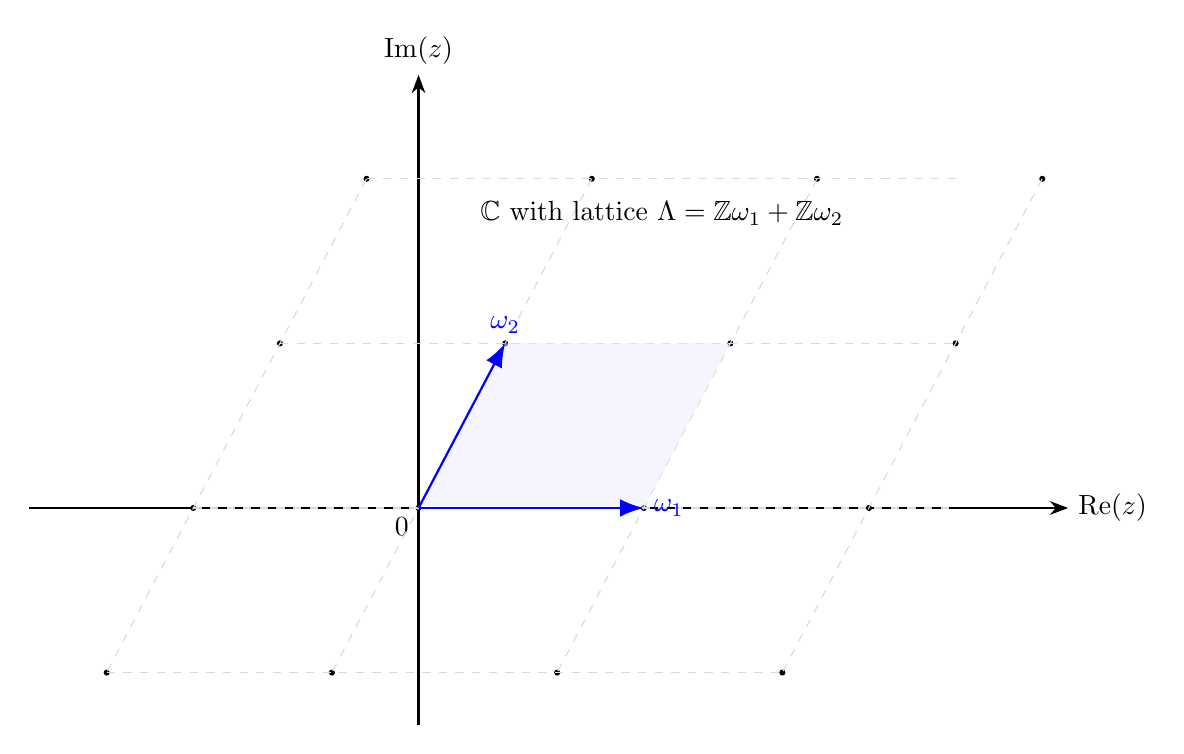
\begin{tikzpicture}[scale=1.1]
	% Parameters for the lattice basis vectors (edit these to taste)
	\def\wone{2.6}      % length of omega_1 along x
	\def\wtwoX{1.0}     % x-component of omega_2
	\def\wtwoY{1.9}     % y-component of omega_2
	
	\draw[-Stealth, thick] (-4.5,0) -- (7.5,0) node[right] {$\Re(z)$};
	\draw[-Stealth, thick] (0,-2.5) to (0,5) node[above] {$\Im(z)$};
	
	% Draw a grid of lattice points around the origin
	\foreach \m in {-1,0,1,2}{
		\foreach \n in {-1,0,1,2}{
			\coordinate (P\m\n) at ({\m*\wone + \n*\wtwoX},{\n*\wtwoY});
			\fill (P\m\n) circle[radius=0.035];
		}
	}
	
	% Origin
	\node[below left] at (0,0) {$0$};
	
%	\foreach \m in {-1,0,1,2}{
%		\foreach \n in {1}{
%			\draw[dashed, gray!30] ({\m*\wone + \n*\wtwoX},{\n*\wtwoY}) -- ({\m*\wone + (-\n)*\wtwoX},{(-\n)*\wtwoY});
%		}
%	}
	\draw[dashed, gray!30] ({-1*\wone + 2*\wtwoX},{2*\wtwoY}) -- ({-1*\wone + (-1)*\wtwoX},{(-1)*\wtwoY});
	\draw[dashed, gray!30] ({0*\wone + 2*\wtwoX},{2*\wtwoY}) -- ({0*\wone + (-1)*\wtwoX},{(-1)*\wtwoY});
	\draw[dashed, gray!30] ({1*\wone + 2*\wtwoX},{2*\wtwoY}) -- ({1*\wone + (-1)*\wtwoX},{(-1)*\wtwoY});;
	\draw[dashed, gray!30] ({2*\wone + 2*\wtwoX},{2*\wtwoY}) -- ({2*\wone + (-1)*\wtwoX},{(-1)*\wtwoY});

%	\foreach \m in {0,1,2}{
%		\foreach \n in {-1,0,1,2}{
%			\draw[dashed, gray!30] ({-\m*\wone + \n*\wtwoX},{\n*\wtwoY}) -- ({(\m)*\wone + \n*\wtwoX},{\n*\wtwoY});
%		}
%	}
	
	\draw[dashed, gray!30] ({-1*\wone + 2*\wtwoX},{2*\wtwoY}) -- ({2*\wone + 1*\wtwoX},{2*\wtwoY});
	\draw[dashed, gray!30] ({-1*\wone + 1*\wtwoX},{1*\wtwoY}) -- ({2*\wone + 1*\wtwoX},{1*\wtwoY});
	\draw[dashed, gray!30] ({-1*\wone + 0*\wtwoX},{0*\wtwoY}) -- ({2*\wone + 1*\wtwoX},{0*\wtwoY});
	\draw[dashed, gray!30] ({-1*\wone + (-1)*\wtwoX},{(-1)*\wtwoY}) -- ({2*\wone - 1*\wtwoX},{(-1)*\wtwoY});
	
	% Fundamental parallelogram
	\coordinate (A) at (0,0);
	\coordinate (B) at (\wone,0);
	\coordinate (C) at ({\wone+\wtwoX},{\wtwoY});
	\coordinate (D) at (\wtwoX,\wtwoY);
	
	\fill[blue!8, opacity=.5] (A)--(B)--(C)--(D)--cycle;
%	\draw[blue!60,very thick] (A)--(B)--(C)--(D)--cycle;
	
	% Basis vectors
	\draw[thick,-{Latex[length=3mm]}, blue] (0,0) -- (\wone,0) node[right] {$\omega_1$};
	\draw[thick,-{Latex[length=3mm]}, blue] (0,0) -- (\wtwoX,\wtwoY) node[above] {$\omega_2$};
	
%	% Labels of edges for identification
%	\draw[blue!60,thick,-{Latex[length=3mm]}] ($(A)!0.5!(B)$) ++(0,0.08) -- ++(0.001,0.001)
%	node[above] {$\sim$};
%	\draw[blue!60,thick,-{Latex[length=3mm]}] ($(D)!0.5!(C)$) ++(0,0.08) -- ++(0.001,0.001)
%	node[above] {$\sim$};
%	
%	\draw[blue!60,thick,-{Latex[length=3mm]}] ($(B)!0.5!(C)$) ++(0.08,0) -- ++(0.001,0.001)
%	node[right] {$\sim$};
%	\draw[blue!60,thick,-{Latex[length=3mm]}] ($(A)!0.5!(D)$) ++(0.08,0) -- ++(0.001,0.001)
%	node[right] {$\sim$};
%	
	% Title
	\node[align=left,anchor=west] at ($(C)+(-3,1.5)$)
	{\(\mathbb{C}\) with lattice \(\Lambda=\mathbb Z\omega_1+\mathbb Z\omega_2\)};
\end{tikzpicture}
\end{document}
